\begin{tikzpicture}[remember picture, scale=\modDGHyperScale]
% dummy
\coordinate[overlay] (v-coord-0-0) at (7.44, 5.731) {};
\coordinate[overlay] (v-coord-1-0) at (3.8694, 5.8056) {};
\coordinate[overlay] (v-coord-2-0) at (9.5767, 1.2528) {};
\coordinate[overlay] (v-coord-3-0) at (4.4234, 1.5254) {};
\coordinate[overlay] (v-coord-5-0) at (1.8463, 0.4714) {};
\coordinate[overlay] (v-coord-4-0) at (7.0548, 2.7973) {};

% id = 0, graphName = GPP
\node[modStyleDGHyperVertex, at=(v-coord-0-0), draw=black] (v-0-0) {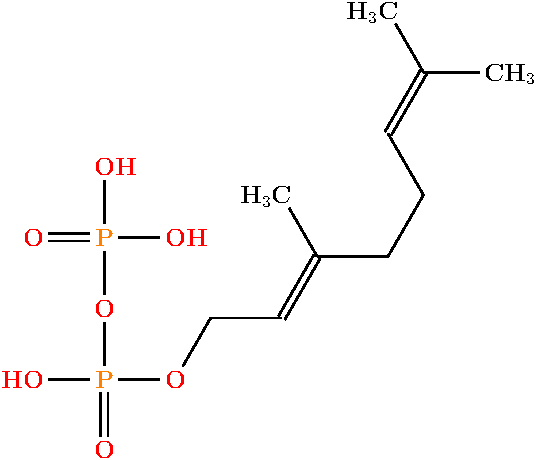
\includegraphics[scale=\modDGHyperImageScale] {\modInputPrefix/out/001_g_0_11311100.pdf}\\{$\mathrm{GPP}$}};
% id = 1, graphName = H2O
\node[modStyleDGHyperVertex, at=(v-coord-1-0), draw=black] (v-1-0) {
\includegraphics[scale=\modDGHyperImageScale] {\modInputPrefix/out/002_g_2_11311100.pdf}\\{$\mathrm{H2O}$}};
% id = 2, graphName = OPP-
\node[modStyleDGHyperVertex, at=(v-coord-2-0), draw=red] (v-2-0) {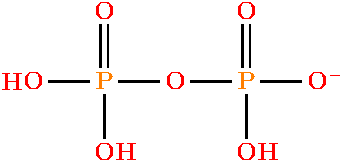
\includegraphics[scale=\modDGHyperImageScale] {\modInputPrefix/out/003_g_3_11311100.pdf}\\{$\mathrm{OPP-}$}};
% id = 3, graphName = geranyl cation C1+
\node[modStyleDGHyperVertex, at=(v-coord-3-0), draw=red] (v-3-0) {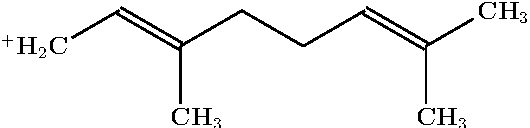
\includegraphics[scale=\modDGHyperImageScale] {\modInputPrefix/out/004_g_4_11311100.pdf}\\{$\mathrm{geranyl\ cation\ C1+}$}};
% id = 5, graphName = p_{0,0}
\node[modStyleDGHyperVertex, at=(v-coord-5-0), draw=red] (v-5-0) {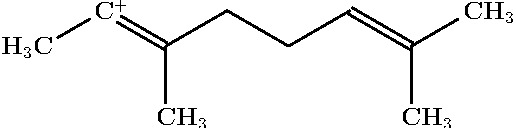
\includegraphics[scale=\modDGHyperImageScale] {\modInputPrefix/out/005_g_41_11311100.pdf}\\{$\mathrm{p_{0,0}}$}};
% id = 4{ 'GPP' }, 'Disphophate loss general', { 'OPP-' 'geranyl cation C1+' }
\node[modStyleDGHyperEdge, at=(v-coord-4-0), draw=red] (v-4-0) {$\mathrm{r_{1}}$};
% id = 4{ 'GPP' }, 'Disphophate loss general', { 'OPP-' 'geranyl cation C1+' }
\path[modStyleDGHyperConnector, draw=black] (v-0-0) to (v-4-0);
\path[modStyleDGHyperConnector, draw=red] (v-4-0) to (v-2-0);
\path[modStyleDGHyperConnector, draw=red] (v-4-0) to (v-3-0);
% id = 6{ 'geranyl cation C1+' }, '1,2 hydrid shift', { 'p_{0,0}' }
\path[modStyleDGHyperConnector, draw=red] (v-3-0) to node[auto, swap] {$\mathrm{r_{0}}$} (v-5-0);
\end{tikzpicture}%
